\documentclass[english, a4paper, 11pt]{article}

\usepackage{microtype}

\usepackage[T1]{fontenc}
\usepackage[utf8]{inputenc}

\usepackage{csquotes}
\usepackage{babel}

\usepackage[bookmarks=true]{hyperref}
\hypersetup{
	pdftitle={Title of the Research Proposal},
	pdfauthor={Author names},
	pdfkeywords={keyword 1, keyword 2},
	bookmarksnumbered,
	breaklinks=true,
	urlcolor=blue,
	citecolor=black,
	colorlinks=true,
	linkcolor=black,
}

\usepackage{lmodern}
\usepackage{amsmath}
\usepackage{amssymb}
\usepackage{textcomp}

\usepackage[style=ieee, citestyle=ieee]{biblatex}
\bibliography{references}

\usepackage[
	per-mode=symbol,
	%output-decimal-marker={,},
	separate-uncertainty=true,
]{siunitx}

\usepackage{booktabs}
\usepackage{caption}
\captionsetup[table]{skip=1ex}

\usepackage{tikz}
\usepackage{graphicx}
\graphicspath{{figures/}}

\usepackage{pgfgantt}

\usepackage{cleveref}

\usepackage[
    % showframe,
	headheight=16mm,
    bottom=30mm,
]{geometry}

\usepackage{fancyhdr}
\fancypagestyle{unicamp}{
\renewcommand{\headrule}{}
\renewcommand{\footrule}{}
\fancyhead{}
\fancyfoot{}
\fancyhead[L]{\definecolor{unicampred}{RGB}{218,41,28}
\begin{tikzpicture}[x=0.08mm, y=0.08mm]
\fill (23.9531, 1.5) arc (3.58332:18.9167:24) -- (68.5957, 26.7897)arc (20.9142:16.5994:265.82) arc (128.381:171.373:10) -- cycle;
\fill (21.5557, 10.5523) arc (26.0833:41.4167:24) -- (55.0392, 52.9179)arc (32.5881:22.0609:144) -- cycle;
\fill (15.8767, 17.998) arc (48.5833:63.9167:24) -- (28.9371, 65.9407)arc (254.14:317.658:10) arc (56.8651:36.5278:55.38) -- cycle;
\fill (7.78063, 22.7038) arc (71.0833:86.4167:24) -- (1.5, 80.0404)arc (89.1258:74.8637:82.58) arc (170.647:236.876:10) -- cycle;
\fill (-1.5, 23.9531) arc (93.5833:108.917:24) -- (-28.6966, 73.1995)arc (115.826:92.2091:68.49) -- cycle;
\fill (-10.5523, 21.5557) arc (116.083:131.417:24) -- (-53.0458, 55.1671)arc (138.056:117.14:75.31) -- cycle;
\fill (-17.998, 15.8767) arc (138.583:153.917:24) -- (-67.7798, 29.6989)arc (162.818:139.707:66.11) -- cycle;
\fill (-22.7038, 7.78063) arc (161.083:176.417:24) -- (-67.7575, 1.5)arc (190.38:172.687:82.03) -- cycle;
\fill (-23.9531, -1.5) arc (183.583:198.917:24) -- (-56.342, -21.714)arc (214.771:200.588:92.45) -- cycle;
\fill (-21.5557, -10.5523) arc (206.083:221.417:24) -- (-38.6627, -36.5413)arc (237.639:225.296:92.84) -- cycle;
\fill (-15.8767, -17.998) arc (228.583:288.917:24) -- (13.0236, -35.3614)arc (118.011:187.497:10) arc (279.181:241.688:69.1) -- cycle;
\fill (10.5523, -21.5557) arc (296.083:311.417:24) -- (33.2593, -35.3806)arc (298.195:295.57:172.01) arc (31.6501:100.731:10) -- cycle;
\fill (17.998, -15.8767) arc (318.583:356.417:24) -- (71.3531, -1.5)arc (188.627:221.289:10) arc (312.84:298.995:193.11) -- cycle;
\fill[unicampred] (31.67, 75.56) circle (7);
\fill[unicampred] (81.24, 0) circle (7);
\fill[unicampred] (17.72, -44.19) circle (7);
\fill (-64, -80) -- (-64, -86.9041) .. controls (-63.9775, -89.3328) and (-63.9775, -89.3328) .. (-63.955, -89.8276) .. controls (-63.8426, -92.0315) and (-63.5952, -92.9535) .. (-62.8531, -93.7181) .. controls (-61.7286, -94.91) and (-59.9295, -95.2249) .. (-54.1949, -95.2249) .. controls (-50.7091, -95.2249) and (-49.2024, -95.1349) .. (-47.8531, -94.8651) .. controls (-46.1439, -94.5052) and (-44.997, -93.3133) .. (-44.7496, -91.6042) .. controls (-44.6147, -90.5472) and (-44.5922, -90.2999) .. (-44.5247, -86.9041) -- (-44.5247, -80) -- (-49.09, -80) -- (-49.09, -86.9041) .. controls (-49.09, -87.2189) and (-49.1124, -87.9385) .. (-49.1349, -88.4558) .. controls (-49.2024, -89.8726) and (-49.3148, -90.2774) .. (-49.6747, -90.6597) .. controls (-50.1694, -91.1994) and (-51.1139, -91.3343) .. (-54.2624, -91.3343) .. controls (-58.1529, -91.3343) and (-59.03, -91.087) .. (-59.2774, -89.8951) .. controls (-59.3898, -89.2879) and (-59.3898, -89.2654) .. (-59.4348, -86.9041) -- (-59.4348, -80) -- (-64, -80);
\fill (-41.2491, -80) -- (-41.2491, -95) -- (-36.5939, -95) -- (-36.7064, -83.8006) -- (-36.2116, -83.8006) -- (-28.3181, -95) -- (-20.3796, -95) -- (-20.3796, -80) -- (-25.0347, -80) -- (-24.9223, -91.1769) -- (-25.3945, -91.1769) -- (-33.2431, -80) -- (-41.2491, -80);
\fill (-17.0509, -80) -- (-17.0509, -95) -- (-12.2608, -95) -- (-12.2608, -80) -- (-17.0509, -80);
\fill (5.3068, -89.2204) .. controls (5.28431, -91.4468) and (5.21684, -91.4693) .. (0.201848, -91.4693) .. controls (-4.61075, -91.4693) and (-4.67821, -91.4243) .. (-4.67821, -87.5787) .. controls (-4.67821, -85.3073) and (-4.4983, -84.4303) .. (-3.95857, -83.9805) .. controls (-3.5088, -83.6207) and (-2.67671, -83.5307) .. (0.17936, -83.5307) .. controls (3.05792, -83.5307) and (4.38476, -83.6657) .. (4.72209, -83.958) .. controls (4.99195, -84.1829) and (5.03693, -84.3853) .. (5.08191, -85.3748) -- (9.64713, -85.3748) -- (9.64713, -84.6327) .. controls (9.64713, -82.2264) and (9.19735, -81.1244) .. (7.91549, -80.4723) .. controls (6.88101, -79.9325) and (5.48671, -79.7751) .. (1.48371, -79.7751) .. controls (-6.36487, -79.7751) and (-8.00655, -80.1574) .. (-8.81614, -82.1814) .. controls (-9.15348, -83.0135) and (-9.24343, -84.2504) .. (-9.24343, -87.6012) .. controls (-9.24343, -89.5127) and (-9.19845, -90.7496) .. (-9.13099, -91.4243) .. controls (-8.95108, -92.9535) and (-8.5013, -93.7856) .. (-7.51179, -94.3478) .. controls (-6.2974, -95.045) and (-4.40835, -95.2249) .. (1.46122, -95.2249) .. controls (4.78956, -95.2249) and (6.43124, -95.09) .. (7.64563, -94.7076) .. controls (9.30979, -94.1679) and (9.93948, -93.066) .. (9.93948, -90.6372) .. controls (9.93948, -90.4123) and (9.91699, -90.075) .. (9.8945, -89.2204) -- (5.3068, -89.2204);
\fill (29.0254, -95) -- (34.2203, -95) -- (26.3717, -80) -- (19.2653, -80) -- (11.3267, -95) -- (16.5441, -95) -- (17.826, -92.4588) -- (27.7435, -92.4588) -- (29.0254, -95) (26.1468, -89.1754) -- (19.4452, -89.1754) -- (22.3462, -83.4858) -- (23.2458, -83.4858) -- (26.1468, -89.1754);
\fill (36.1297, -80) -- (36.1297, -95) -- (40.6275, -95) -- (40.515, -83.7781) -- (41.3246, -83.7781) -- (46.9693, -95) -- (50.7699, -95) -- (56.4146, -83.7781) -- (57.1792, -83.7781) -- (57.0668, -95) -- (61.5645, -95) -- (61.5645, -80) -- (53.3336, -80) -- (48.8584, -89.7376) -- (44.4056, -80) -- (36.1297, -80);
\fill (64.896, -95) -- (69.4612, -95) -- (69.4612, -91.3343) -- (75.2183, -91.3343) .. controls (78.4567, -91.3343) and (79.4687, -91.2444) .. (80.4807, -90.907) .. controls (82.2798, -90.2549) and (82.887, -88.9505) .. (82.887, -85.6222) .. controls (82.887, -81.7766) and (82.0774, -80.5622) .. (79.2438, -80.1349) .. controls (78.4117, -80.0225) and (78.0069, -80) .. (75.1733, -80) -- (64.896, -80) -- (64.896, -95) (69.4612, -87.5787) -- (69.4612, -83.7556) -- (75.1733, -83.7556) .. controls (77.1748, -83.7781) and (77.2198, -83.7781) .. (77.5347, -83.8906) .. controls (78.1194, -84.093) and (78.3218, -84.5427) .. (78.3218, -85.6222) .. controls (78.3218, -86.6567) and (78.1868, -87.0615) .. (77.7596, -87.3313) .. controls (77.3772, -87.5562) and (77.2873, -87.5562) .. (75.1733, -87.5787) -- (69.4612, -87.5787);
\end{tikzpicture}
}
\fancyhead[C]{\sffamily%
{\bfseries\fontsize{15.5pt}{1em}\selectfont\uppercase{Universidade Estadual de Campinas}}\\
\fontsize{11.3pt}{1.2em}\selectfont\uppercase{Faculdade de Engenharia Elétrica e de Computação}\\
}
\fancyfoot[C]{\sffamily\fontsize{9pt}{1em}\selectfont%
Av. Albert Einstein, 400; 13083-852 Campinas, SP, Brasil\\
Tel: +55 (19) 3521-3703; Fax: +55 (19) 3289-1395\\
\url{http://www.fee.unicamp.br}}
}

\pagestyle{plain}

\usepackage{setspace}

%\usepackage{parskip}

\usepackage{relsize}
\usepackage[nomain, acronym]{glossaries}
\setacronymstyle{long-sm-short}
\newcommand{\newacronymx}[8][]{%
	\newglossaryentry{#2}{
	type=\acronymtype,
	name={{\smaller #3}},
	sort={#3},
	first={#4 ({\smaller #3}, \emph{#5})},
	firstplural={#7 ({\smaller #6}, \emph{#8})},
	text={{\smaller #3}},
	plural={{\smaller #6}},
	description={#4 (\emph{#5})},#1}}

\newacronym{RTFM}{RTFM}{read the freaking manual}
\newacronymx{AOL}{AOL}{acronym in another language}{acrônimo em outra língua}{AOLs}{acronyms in another language}{acrônimos em outra língua}


\begin{document}

\thispagestyle{unicamp}

\begin{center}

    
\includegraphics[width=0.7\linewidth]{logo-syrte.png}
    
\null\vfill

{\scshape\large Project EA006 - Trabalho de Fim de Curso \par}

\vskip 3\baselineskip

{\LARGE\bfseries Delta Kick Squeezing for Atom
Interferometry beyond the Standard
Quantum Limit\par}

\vskip 3\baselineskip

Candidate:\\[1ex]
{\large\bfseries Daniel Gonçalves Benvenutti\par}
{\large danielgb23@gmail.com\par}
{\large d169448@unicamp.br\par}
{\large RA: 169448\par}

\vskip 3\baselineskip

Advisor:\\[1ex]
{\large\bfseries José Alexandre Diniz\par}
{\large jadiniz@unicamp.br\par}

\end{center}

\vfill
\clearpage

%\section*{guidelines delete later}
%Para ter a matrícula atendida é necessário submeter, via SIGA, os seguintes documentos em um único arquivo pdf:
%
%– Plano de Trabalho, devidamente assinados pelo(a) estudante e pelo(a) orientador(a)/coorientador(a) do projeto
%
%– Formulário para Apresentação do Plano de Trabalho  devidamente preenchido e assinado pelo(a) estudante e orientador(a)/coorientador(a)
%
%OBS.  As solicitações de matrícula somente serão aceitas mediante entrega do plano de trabalho e do formulário.
%
%Sugestão de formato de Plano de Trabalho:
%
%Capa: Sigla e nome da disciplina; Título do trabalho; RA, nome completo, e-mails  do(a) estudante; Nome completo do orientador(a)/coorientador(a); e-mail e unidade de ensino (somente aos orientadores externos à FEEC).
%
%Corpo:
%Introdução: caracterização do problema com citações bibliográficas;
%Objetivos: detalhar os objetivos específicos do trabalho para o período proposto;
%Descrição das etapas a serem cumpridas e dos métodos e técnicas a serem utilizados;
%Cronograma;
%Documentos opcionais: quando for o caso, apresentar outros documentos como orçamento, aprovação pelo Comitê de Ética em Pesquisa, etc.;
%Bibliografia: apresentar bibliografia detalhada.
%
%\url{https://www.fee.unicamp.br/graduacao/tfc/}
%
%\onehalfspacing

\section{Introduction}

%Our team at SYRTE develops inertial sensors (gyrometers, accelerometers...) based on atom interferometry technics. The development of these instruments benefits from the maturity of ultracold atom technology and the advantage of light beamsplitters, easy to implement and efficient, namely two photon transitions and more specifically stimulated Raman transitions. If these methods allow now for the development of commercial products with applications in geophysics on the field, and of onboard instruments in ships or planes for inertial navigation and geoscience, increasing significantly the performances of such instruments remains possible, in particular by using advanced quantum metrology methods to surpass the standard quantum limit.

%The aim of this intership is the implementation of the "Delta-Kick squeezing" (DKS) technique, recently proposed by Robin Corgier, currently a postdoctoral fellow at SYRTE, and his collaborators. This DKS rely on the engineering of atom atom interactions in a BEC in free fall. Such interactions induce strong correlations between the atoms, and lead to squeezing in the population difference between the two interferometer paths, and eventually to phase sensitivity below the standard quantum limit.

%The intern will work on implementing this method in a free-falling atom interferometer, based on the use of Raman light beamsplitters and ultra-cold atoms produced by evaporative cooling. The work, essentially experimental in nature, will first consist in optimizing the preparation sequence of ultra-cold atoms, to obtain Bose Einstein condensates in a robust and efficient way, and in optimizing the detection method of the two output ports of the interferometer. The intern will then demonstrate the possibility of realizing strongly spin-squeezed states through atomic lensing methods based on pulse sequences realized with highly detuned high power laser beams. Finally, he or she will study the impact of the use of these quantum states in an interferometer on the sensitivity of measurements. He or she will conduct the experimental studies and participate in the analysis of the results. He or she will have extensive theoretical support for the modeling of the experiment, the optimization of the measurement sequence and for the analysis of the results.

In this final dissertation (TFC) for the subject EE006 the student will work  full time for 12 weeks at the laboratory SYRTE (Systèmes de Référence Temps-Espace), located in Paris, a department of the Observatoire de Paris, a member of the PSL Research University. The final dissertation will be a report written in the form of a scientific article about the work done there. 

The Observatoire de Paris is a public institution dedicated to fundamental and applied research, higher education and the sharing of knowledge in disciplines related to physics and astrophysics, history of science and astronomy. It offers research-based teaching from bachelor's to doctorate level, as well as university diplomas and training courses for teachers. Highly involved in knowledge sharing, the establishment offers educational resources for all levels and ages (class sponsorship, exhibitions, digital media, etc.) and takes part in numerous events (Fête de la Science, etc.). (\href{https://www.observatoiredeparis.psl.eu/-observatoire-de-paris-.html?lang=fr}{site})

The SYRTE laboratory develops inertial sensors (gyrometers, accelerometers...) based on atom interferometry technics. The development of these instruments benefits from the maturity of ultracold atom and quantum optics technologies. Atom interferometry works by splitting the wave function of an atom into a superposition of two wavepackets with different momenta. These two partial wavepackets then propagate along two different paths which constitute the two interferometer arms, before getting recombined, leading to interferences. The interaction with the gravitational field leads to an interferometer phase shift, arising from the difference of phases accumulated along the two paths. To manipulate the atomic wavepackets, we can use light beamsplitters, easy to implement and efficient, and in particular at SYRTE two photon transitions, more specifically stimulated Raman transitions. 

Increasing significantly the performances of such instruments by getting grants to do more research remains possible, given that these methods allow now for the development of commercial products with applications in geophysics on the field and of onboard instruments in ships or planes for inertial navigation and geoscience. 

We can increase this performance in particular by using advanced quantum metrology methods to surpass the standard quantum limit.
The technique that will be implemented to surpass this limit is called  "Delta-Kick squeezing" (DKS), as proposed in \cite{Corgier_2021}.
%recently proposed by Robin Corgier, currently a postdoctoral fellow at SYRTE, and his collaborators. 

\subsection{Cold/Ultra cold Atoms}
%\url{https://hal.science/hal-01166054/document}
This field in short works by controlling groups or even individual atoms in a vacuum chamber. Both the internal degrees of freedom like the excitation (deexcitation) of an electron to a higher (lower) energy state within the atom and, what is very notable, the external degrees of freedom of an atom like it's momentum and position.


This relationship between the external degrees of freedom and light is given because light has momentum and that momentum can be transferred to an atom. Under the right conditions we can transfer momentum away from the atoms effectively stopping and therefore cooling them in 3 dimensions.

One way of doing that is using Doppler cooling. We direct the lasers at the atom on the direction that we want to slow them and with a frequency that is slightly lower than the atomic resonance. When an atom moves opposite to the direction of propagation of the laser, the Doppler shift brings the laser onto resonance, and the atom efficiently absorb photons from the laser beam that slow it down.

Another way is using magneto-optical traps (MOT) that shift the energy levels towards or away from the laser by using a magnetic field gradient. This magnetic field splits the atomic transition into it's Zeeman components which couple with the different modes of circularly polarized light. The splitting depends on the amplitude of the magnetic field and therefore of the position of the atom because of the gradient. We can then shine lasers with different polarizations into opposite directions keeping the atoms in place and cooling then simultaneously.

We can also use optical tweezers which are lasers focused on a single point in 3D space to keep an atom in a location as well as move it around. These tweezers' light generate a trapping potential in which the atom is confined.

This signifies that we can have some or even individual atoms in a vacuum chamber with their degrees of freedom controlled by light given the advancement of laser technologies. There are many possibilities to what can be done. We can use lasers to control their internal states and build atomic clocks which will output a frequency of light defined by atoms that are always the same everywhere, we can also use these atoms individually as qubits and do quantum computations\cite{scholl2021simulation} and we can cool down atoms enough and with enough proximity so that their De Brooglie wavelengths overlap and they form Bose-Einstein condensates
\cite{fallani2015cold}.

\subsection{Atom Interferometry and gravimetry}
Atom interferometers are versatile tools allowing to measure accelerations and rotations with absolute accuracy and high stability\cite{geiger2020highaccuracy}. They are used in fundamental physics to conduct quantum tests of the Einstein equivalence principle\cite{asenbaum2020atom}, measure fundamental constants\cite{rosi2014precision},\cite{morel2020determination}, pose limits on Dark Energy models\cite{elder2016chameleon}, or detect Casimir forces. With increasing technical maturity and size reduction, they are now used as in-field devices for terrestrial absolute gravimetry\cite{menoret2018gravity} and are becoming important tools for the study of the climate system. The first atom-interferometric experiments on board of sounding rockets\cite{becker2018space}, the International Space Station\cite{aveline2020observation} and the development of the satellite-based atom interferometry pathfinder CARIOQA\cite{lévèque2022carioqa} for the study of the climate system demonstrate the potential and importance of this research field. There are also proposals of atom interferometry to detect gravitational waves\cite{badurina2022prospective}.

The interferometer works in the following fashion. It consists of a sequence of three Raman laser pulses $\pi/2$ - $\pi$ - $\pi/2$ , each separated by a free-evolution time T. The three pulses are performed with the same laser intensities but with durations respectively of: $\tau/2$ - $\tau$ - $\tau/2$ . The first pulse separates the atoms' wavefunction into a coherent superposition between the two hyperfine states, by transferring the momentum of two photons to one of the two states. During the first interval T of free evolution, the two arms of the interferometer separate. The second pulse acts on both arms of the interferometer, exchanging the hyperfine levels of the two wave packets and their velocities. As a result of the $\pi$ pulse, the two wave packets come closer together and overlap after a second time interval T . Finally, the last $\pi/2$ pulse recombines the two arms of the interferometer so that they interfere (see figure \ref{fig:interf})
\cite{cheinet2006conception}.

\begin{figure}
    \centering
    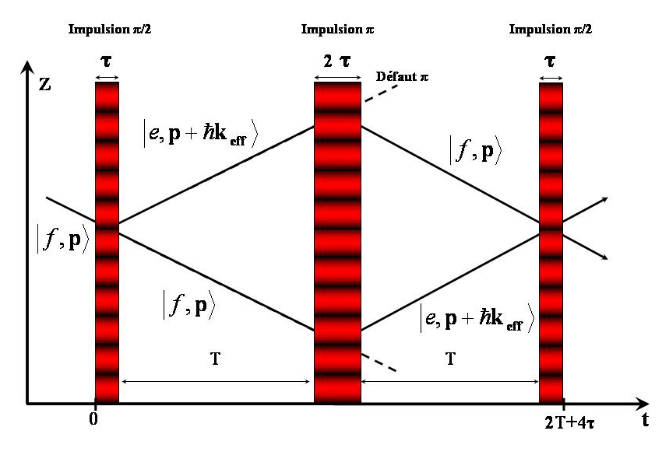
\includegraphics[width=1\linewidth]{figures/interferometry.png}
    \caption{Adapted from \cite{cheinet2006conception}. Schematics of the atom interferometry with Raman pulses in red.}
    \label{fig:interf}
\end{figure}

The atomic levels then can be selectively detected with fluorescence. The probability of detecting the excited hyperfine state is given by:
\begin{equation}
P_e(2T+2\tau)= \frac{1- A\cos(\overrightarrow g\cdot \overrightarrow k_{\mathrm{eff}}T^2)}{2}
\end{equation}
Where $g$ is the acceleration of gravity, $k_{\mathrm{eff}}$ is given by the difference in momentum of the two lasers $\hbar \overrightarrow k_{\mathrm{eff}}= \hbar(\overrightarrow k_1-\overrightarrow k_2)$ and $A$ the contrast. From this transition probability, we can deduce $g$\cite{dos2008gravimetre}.

%\urf{https://metrologie-francaise.lne.fr/sites/default/files/media/document/p33-40-rfm13-pereira-gravimetre-atomes-froids.pdf}


%\url{https://theses.hal.science/tel-00070861}
\subsection{Squeezing}
In quantum mechanics we have the Heisenberg uncertainty principle that gives us the relationship for two non-commuting conjugate variables.  For example position (X) and momentum (P):
\begin{equation}
    \Delta X \Delta P \ge \frac{\hbar}{2}
    \label{eq:saymyname}
\end{equation}
Or also for time (t) and energy (E). A coherent state, where there's minimum uncertainty, satisfies the  condition 
\begin{equation}
    \Delta X = \Delta P = \sqrt{\frac{\hbar}{2}}
\end{equation}
The uncertainty  principle in equation \ref{eq:saymyname} cannot be violated. But we can choose a state to make $\Delta X$ or $\Delta P$ smaller than $\sqrt{\hbar/2}$, a state called a coherent squeezed state where we trade uncertainty in one variable for uncertainty in it's conjugate variable
%\url{https://arxiv.org/pdf/1011.2978.pdf}
\cite{Ma_2011}. 


For our case, the conjugate variables are the phase estimation of the interferometer and the population difference between the two output ports of the interferometer. This would be analogous to the phase and photon number in a light interferometer. The aim is reducing the uncertainty in the phase estimation.

\subsection{Delta-Kick squeezing (DKS)}
%This DKS rely on the engineering of atom atom interactions in a BEC in free fall. Such interactions induce strong correlations between the atoms, and lead to squeezing in the population difference between the two interferometer paths, and eventually to phase sensitivity below the standard quantum limit.
The phase estimation uncertainty for atom interferometers is lower bounded by the standard quantum limit (SQL), $\Delta \theta_{SQL} = 1/\sqrt{N}$, where N is the uncorrelated number of atoms in the interferometer.
By squeezing the phase estimation, this limitation is overcome with the DKS method proposed to enhance the generation of entanglement in free-fall atom-interferometers using atom-atom interactions within Bose Einstein condensates (BECs).  

The key idea consists in focusing the matter-waves through the rapid application of an external trapping potential in analogy to optics, where the trap plays the role of a converging lens. Going through the focal point increases the matter-wave density and thus the effective strength of the particle-particle interactions preparing the atoms in a highly-entangled spin-squeezed state. Considering previous works on delta-kick collimation, the team designate the technique delta-kick squeezing (DKS)
%\url{https://arxiv.org/pdf/2103.10896.pdf}
\cite{Corgier_2021}.

\section{Objectives}

The aim of this internship is to support in the implementation of the "Delta-Kick squeezing" (DKS) technique by improving the power of the current Raman Laser excitation system and inserting this new system into the interferometry setup. This will allow the intern to learn about the experimental implementation of laser optics and systems while maintaining contact with the procedures of the experiment and its underlying concepts. This will give a good basis to work in the field of cold atoms and experimental quantum mechanics. The preparation of the final report will also permit the intern to learn and improve his skills into producing valuable documentation that can facilitate the reproduction of the procedures implemented.

%The extra power will be necessary for

\section{Methodology}


\subsection{Stimulated Raman Transition}
To make an atom interferometer it's necessary to create a coherent superposition of two quantum states of an atom and then recombine the wave packets. An electromagnetic transition can achieve this superposition, while transferring the photon's momentum to the second quantum state. The two states then have different momenta and the interferometer will be sensitive to inertial forces.

The two quantum states must have a long lifetime in relation to the duration of the experiment. In the case of alkaline atoms (in our setup Rb-87), the two hyperfine sublevels of the ground state can be used
\cite{cheinet2006conception}.

We don't excite the atom between these two levels directly. For that we'd need to implement microwaves in our setup whose photons have a very small momentum and would lead to a tiny atom interferometer with an also small sensitivity. 
We do instead a two photon transition with lasers with an wavelength near 780nm. By using a two photon transition these levels can be coupled directly as shown in figure \ref{fig:levels}.
%What we actually do is combining two lasers that, one, excite from the ground to a much higher state. And the other deexcites the atom to the hyperfine state. Both with a large detuning from the higher intermediate state so that we don't get any significant population and neither spontaneous emissions from this level figure \ref{fig:levels}.

\begin{figure}
    \centering
    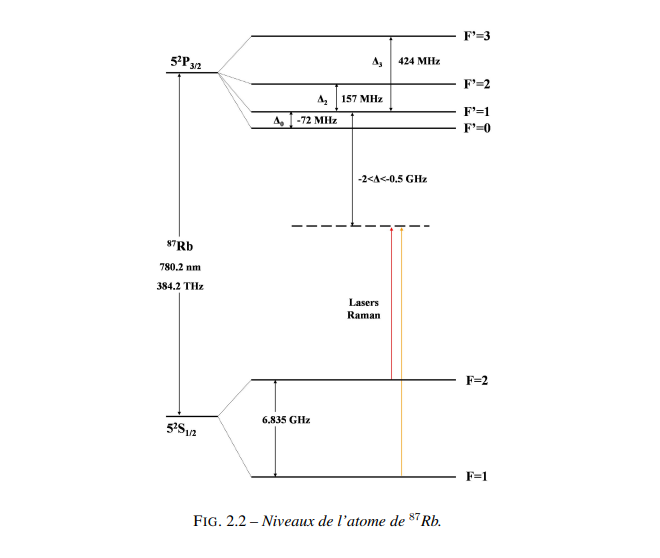
\includegraphics[width=1\linewidth]{figures/raman-levels.png}
    \caption{$^{87}$Rb levels with raman lasers transitions and detuning $\Delta$. Adapted from \cite{cheinet2006conception}.}
    \label{fig:levels}
\end{figure}

The input lasers for the Raman presently available do not have enough power to properly excite the atoms. Therefore we need to amplify them and for that the intern will use a tapered amplifier (TA) that can amplify both wavelengths at the same time. 

The main issue we encounter with the TA is that its output is astigmatic. This means the beam does not focus in the same place in each of the axis transversal to the propagation (vertical and horizontal). Thus we need to use a combination of lenses, one of them spherical and one  cylindrical, to correct this. Other corrections might also be needed to match the mode of the fiber and get optimal coupling.

Afterwards we take the board with the amplifier setup and implement it in the experiment, verify that all systems are functioning properly and test it with the Mach-Zehder interferometer and the atoms in the chamber.

%\textcolor{red}{how do I plan to implement the new Raman}

%The intern will work on implementing this method in a free-falling atom interferometer, based on the use of Raman light beamsplitters and ultra-cold atoms produced by evaporative cooling. The work, essentially experimental in nature, will first consist in optimizing the preparation sequence of ultra-cold atoms, to obtain Bose Einstein condensates in a robust and efficient way, and in optimizing the detection method of the two output ports of the interferometer. The intern will then demonstrate the possibility of realizing strongly spin-squeezed states through atomic lensing methods based on pulse sequences realized with highly detuned high power laser beams. Finally, he or she will study the impact of the use of these quantum states in an interferometer on the sensitivity of measurements. He or she will conduct the experimental studies and participate in the analysis of the results. He or she will have extensive theoretical support for the modeling of the experiment, the optimization of the measurement sequence and for the analysis of the results.
\section{Schedule of Activities}
The activities planned for the intern are the following:

\begin{enumerate}
    \item  Setting up of an amplifier system using tapered amplifiers (TA) for the Raman laser system

\item Beam alignment and shaping for high coupling efficiency into optical fiber after TA + Isolator

\item Transfer of module into experimental setup/main laser system

\textbf{Modifications of main laser system:}

\item Couple the two Raman lasers into the new module via optical fibers

\item (Amplification in the new module and overlap of both beams)
 
 \item Implement laser frequency phase lock loop (PLL) at 6.8 GHz (Raman transition for Rb-87)
 
 \item Implement into software framework (check control of shutters, AOMs etc.)

 \item  Test of system by using the atoms and implementing a simple Mach-Zehnder Interferometer with Raman pulses.

 \item Writing report
\end{enumerate}

The proposed schedule of activities for the project is presented in the Gantt chart in \cref{fig:gantt}.

\begin{figure}[thp]
\centering
\begin{ganttchart}[
hgrid=true,
vgrid=true,
canvas/.append style={draw=none},
title/.append style={draw=none},
title label font=\small,
bar label font=\small,
y unit title=5mm,
y unit chart=6mm,
x unit=8mm,
]{1}{12}
\gantttitle{April}{1}
\gantttitle{May}{3}
\gantttitle{June}{7}
\gantttitle{July}{1}\\
\gantttitlelist{1,...,12}{1}\\
\ganttbar{1.}{1}{1}\\
\ganttbar{2.}{2}{2}\\
\ganttbar{3.}{3}{3}\\
\ganttbar{4.}{4}{4}\\
\ganttbar{5.}{5}{6}\\
\ganttbar{6.}{7}{8}\\
\ganttbar{7.}{9}{10}\\
\ganttbar{8.}{11}{12}\\
\ganttbar{9.}{9}{12}
\end{ganttchart}
\caption{Schedule of activities in weeks.}
\label{fig:gantt}
\end{figure}

%\section{Conclusion}

\printbibliography

\end{document}
